\section{Playing time estimation}
\textit{Sophie's Flying Castle: Dungeons and Djinns} playing time is supposed to be 6 hours for the main story and 10-11 for the 100\% completion.

\textit{In enemy territory} is one of the longest levels of the game, due to its wide map, the high number of interactions with enemies and NPCs and, also, of cutscenes.

We have supposed that cutscenes, pathing inside the castle and puzzles have a fixed time because the average time taken to complete them will be more or less the same for the greater part of the players. But, in order to calculate the total time taken, we have considered three different possible paths within the city of Dynamia:
\begin{itemize}
\item \textbf{Shortest path}: the player doesn't care about exploring the map and he will go from checkpoint to checkpoint using the shortest possible path.
\item \textbf{Average path}: the player will explore a wider area, looking for some rewards near the points of interest, but he will not lose too much time looking for all of the rewards
\item \textbf{Longest path}: the player will roam around the city until he will have found every reward/collectable.
\end{itemize}
\textbf{Cutscenes time}: $\sim$12 minutes.

\textbf{Puzzles solving/fighting time}: $\sim$30 min (4-6 min avg. time for each puzzle and 2-3 minutes avg. for each enemy , excluded the captain part that is supposed to last 7-10 minutes).

\textbf{Pathing time inside the castle}: $\sim$7 min (given that there are few rewards to find and given that the player will have to walk for about 350 m at a very slow pace, $\sim$3 km/h, due to the presence of enemies).

\textbf{Pathing time outside the castle}, assuming an average speed on the ground of 14 km/h (walking 8 km/h, running 20 km/h) and 30 km/h on the sea, while using the magic gondola:
\begin{figure}[H]
    \centering
	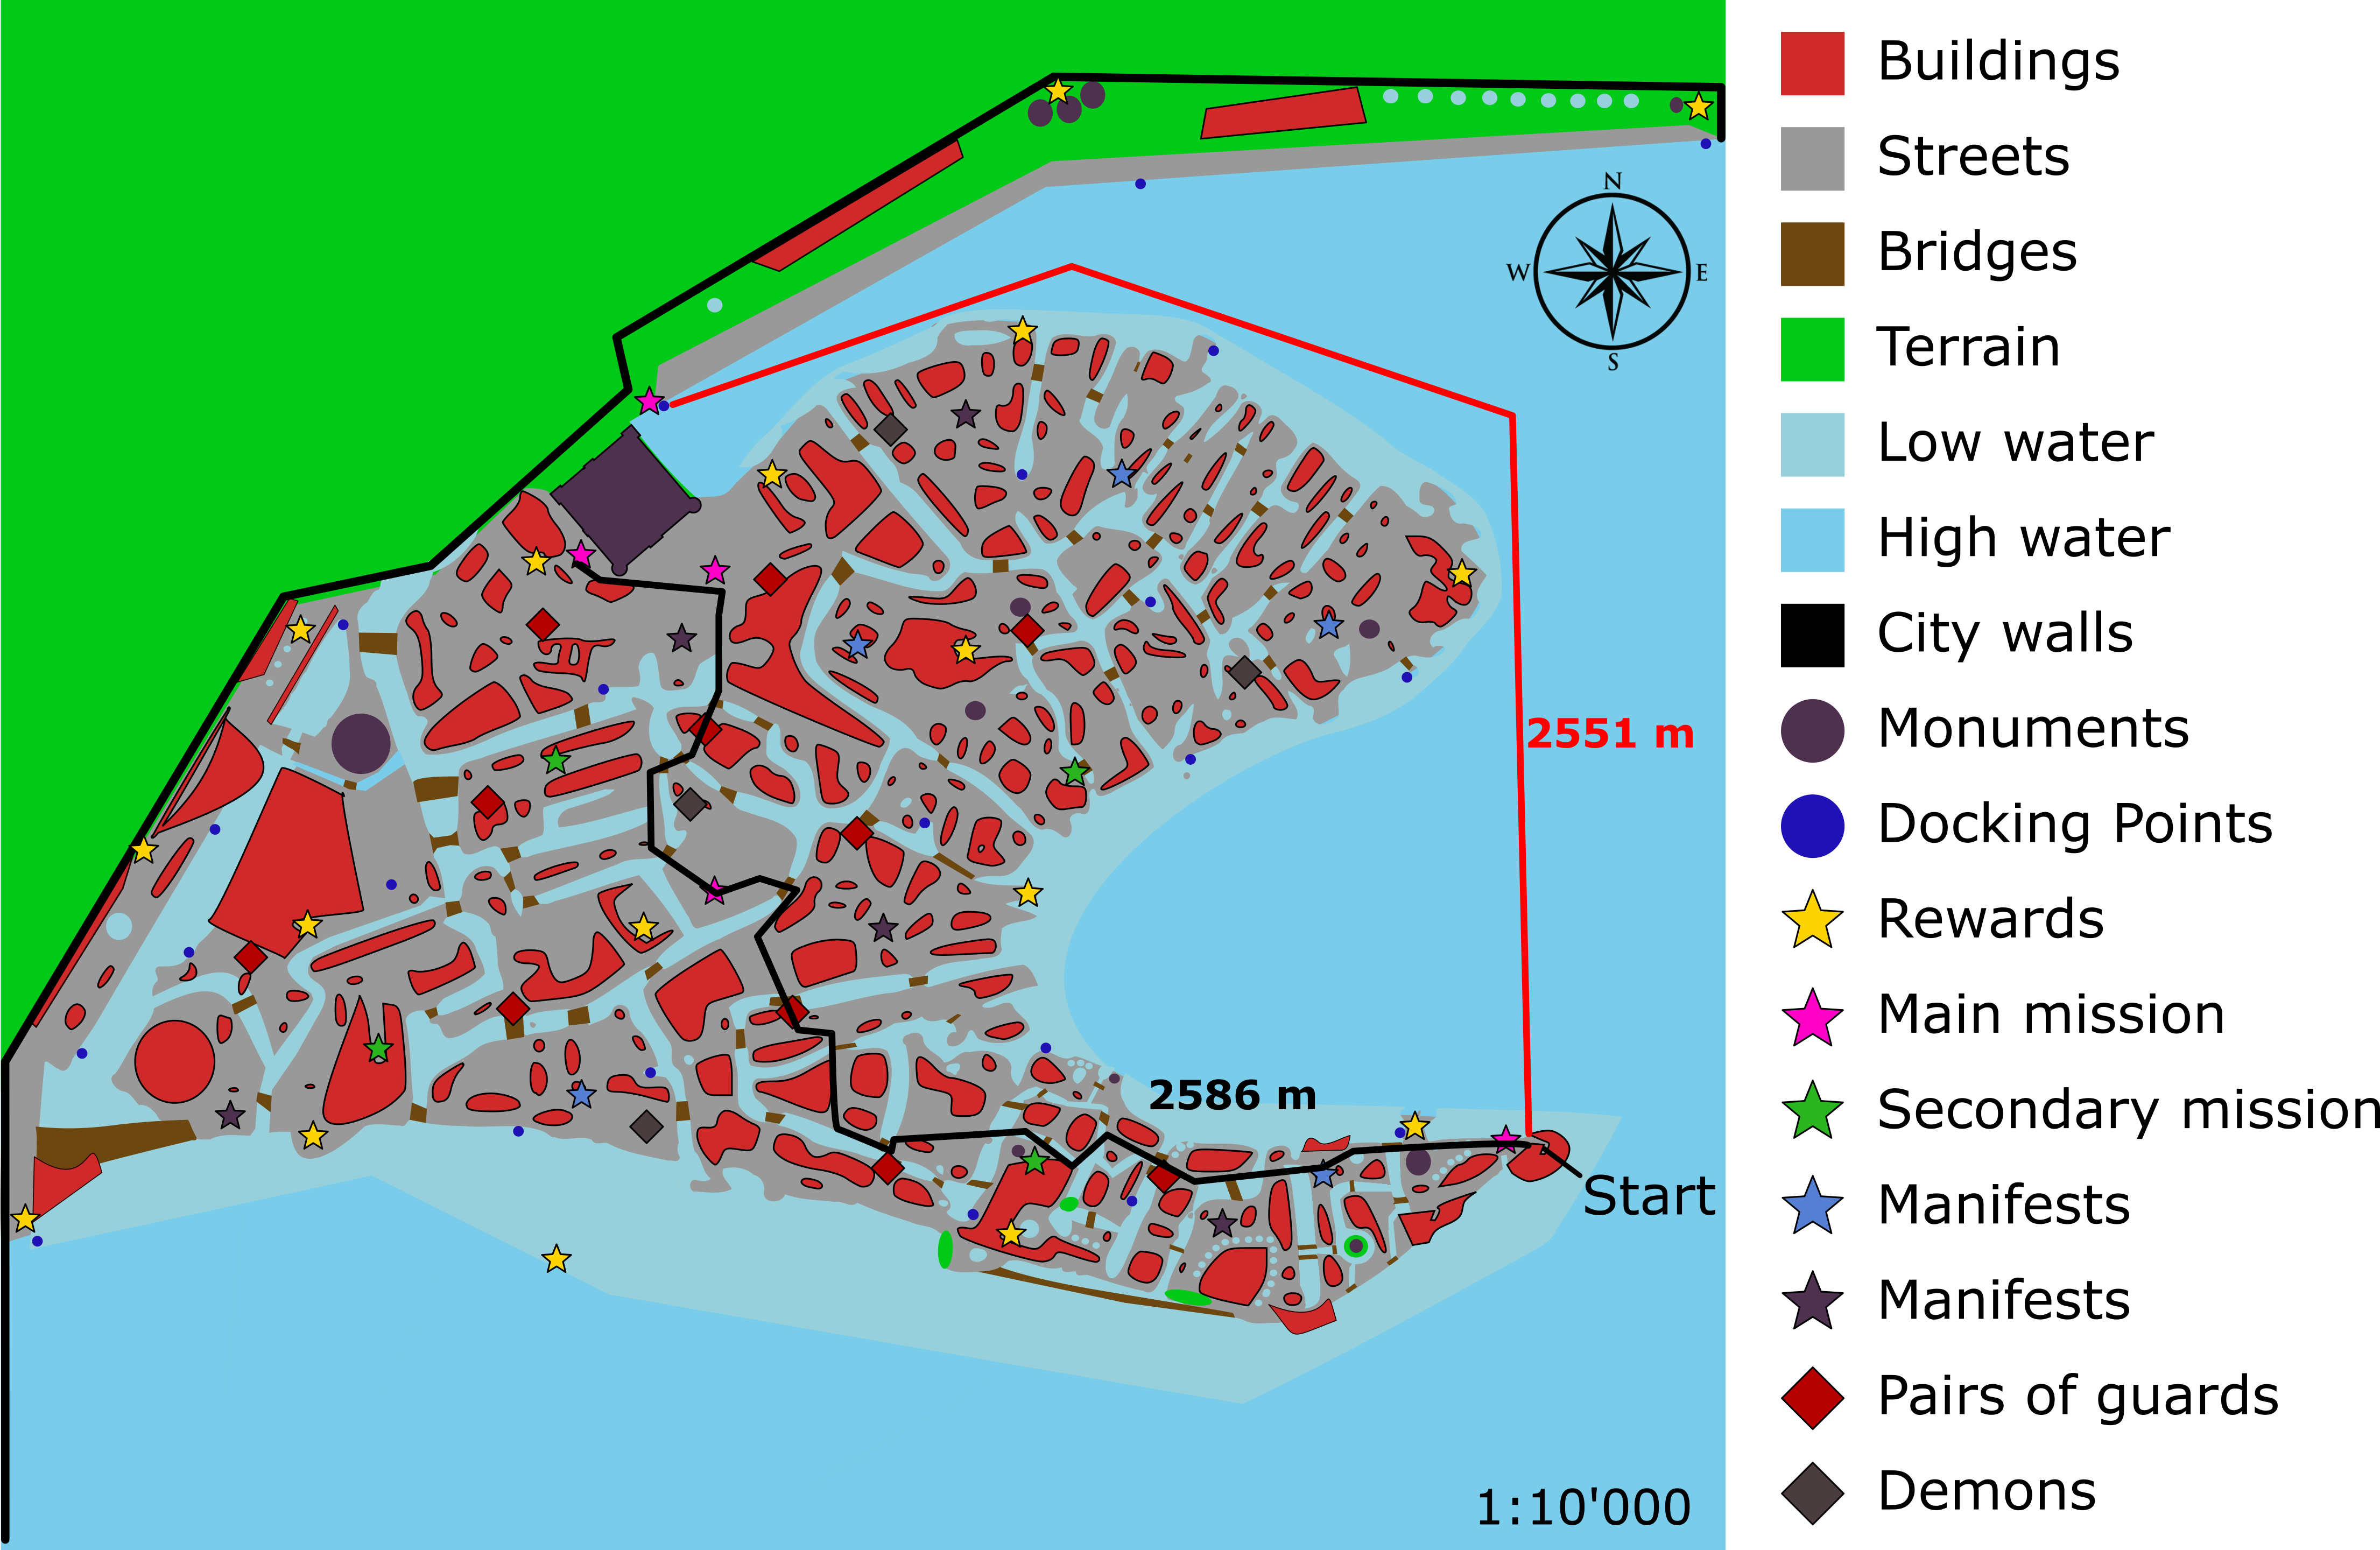
\includegraphics[width=\textwidth]{Images/Diagrams/dynamiapath1.png}
	\caption{Shortest path: $\sim$16 min}
\end{figure}

\begin{figure}[H]
    \centering
	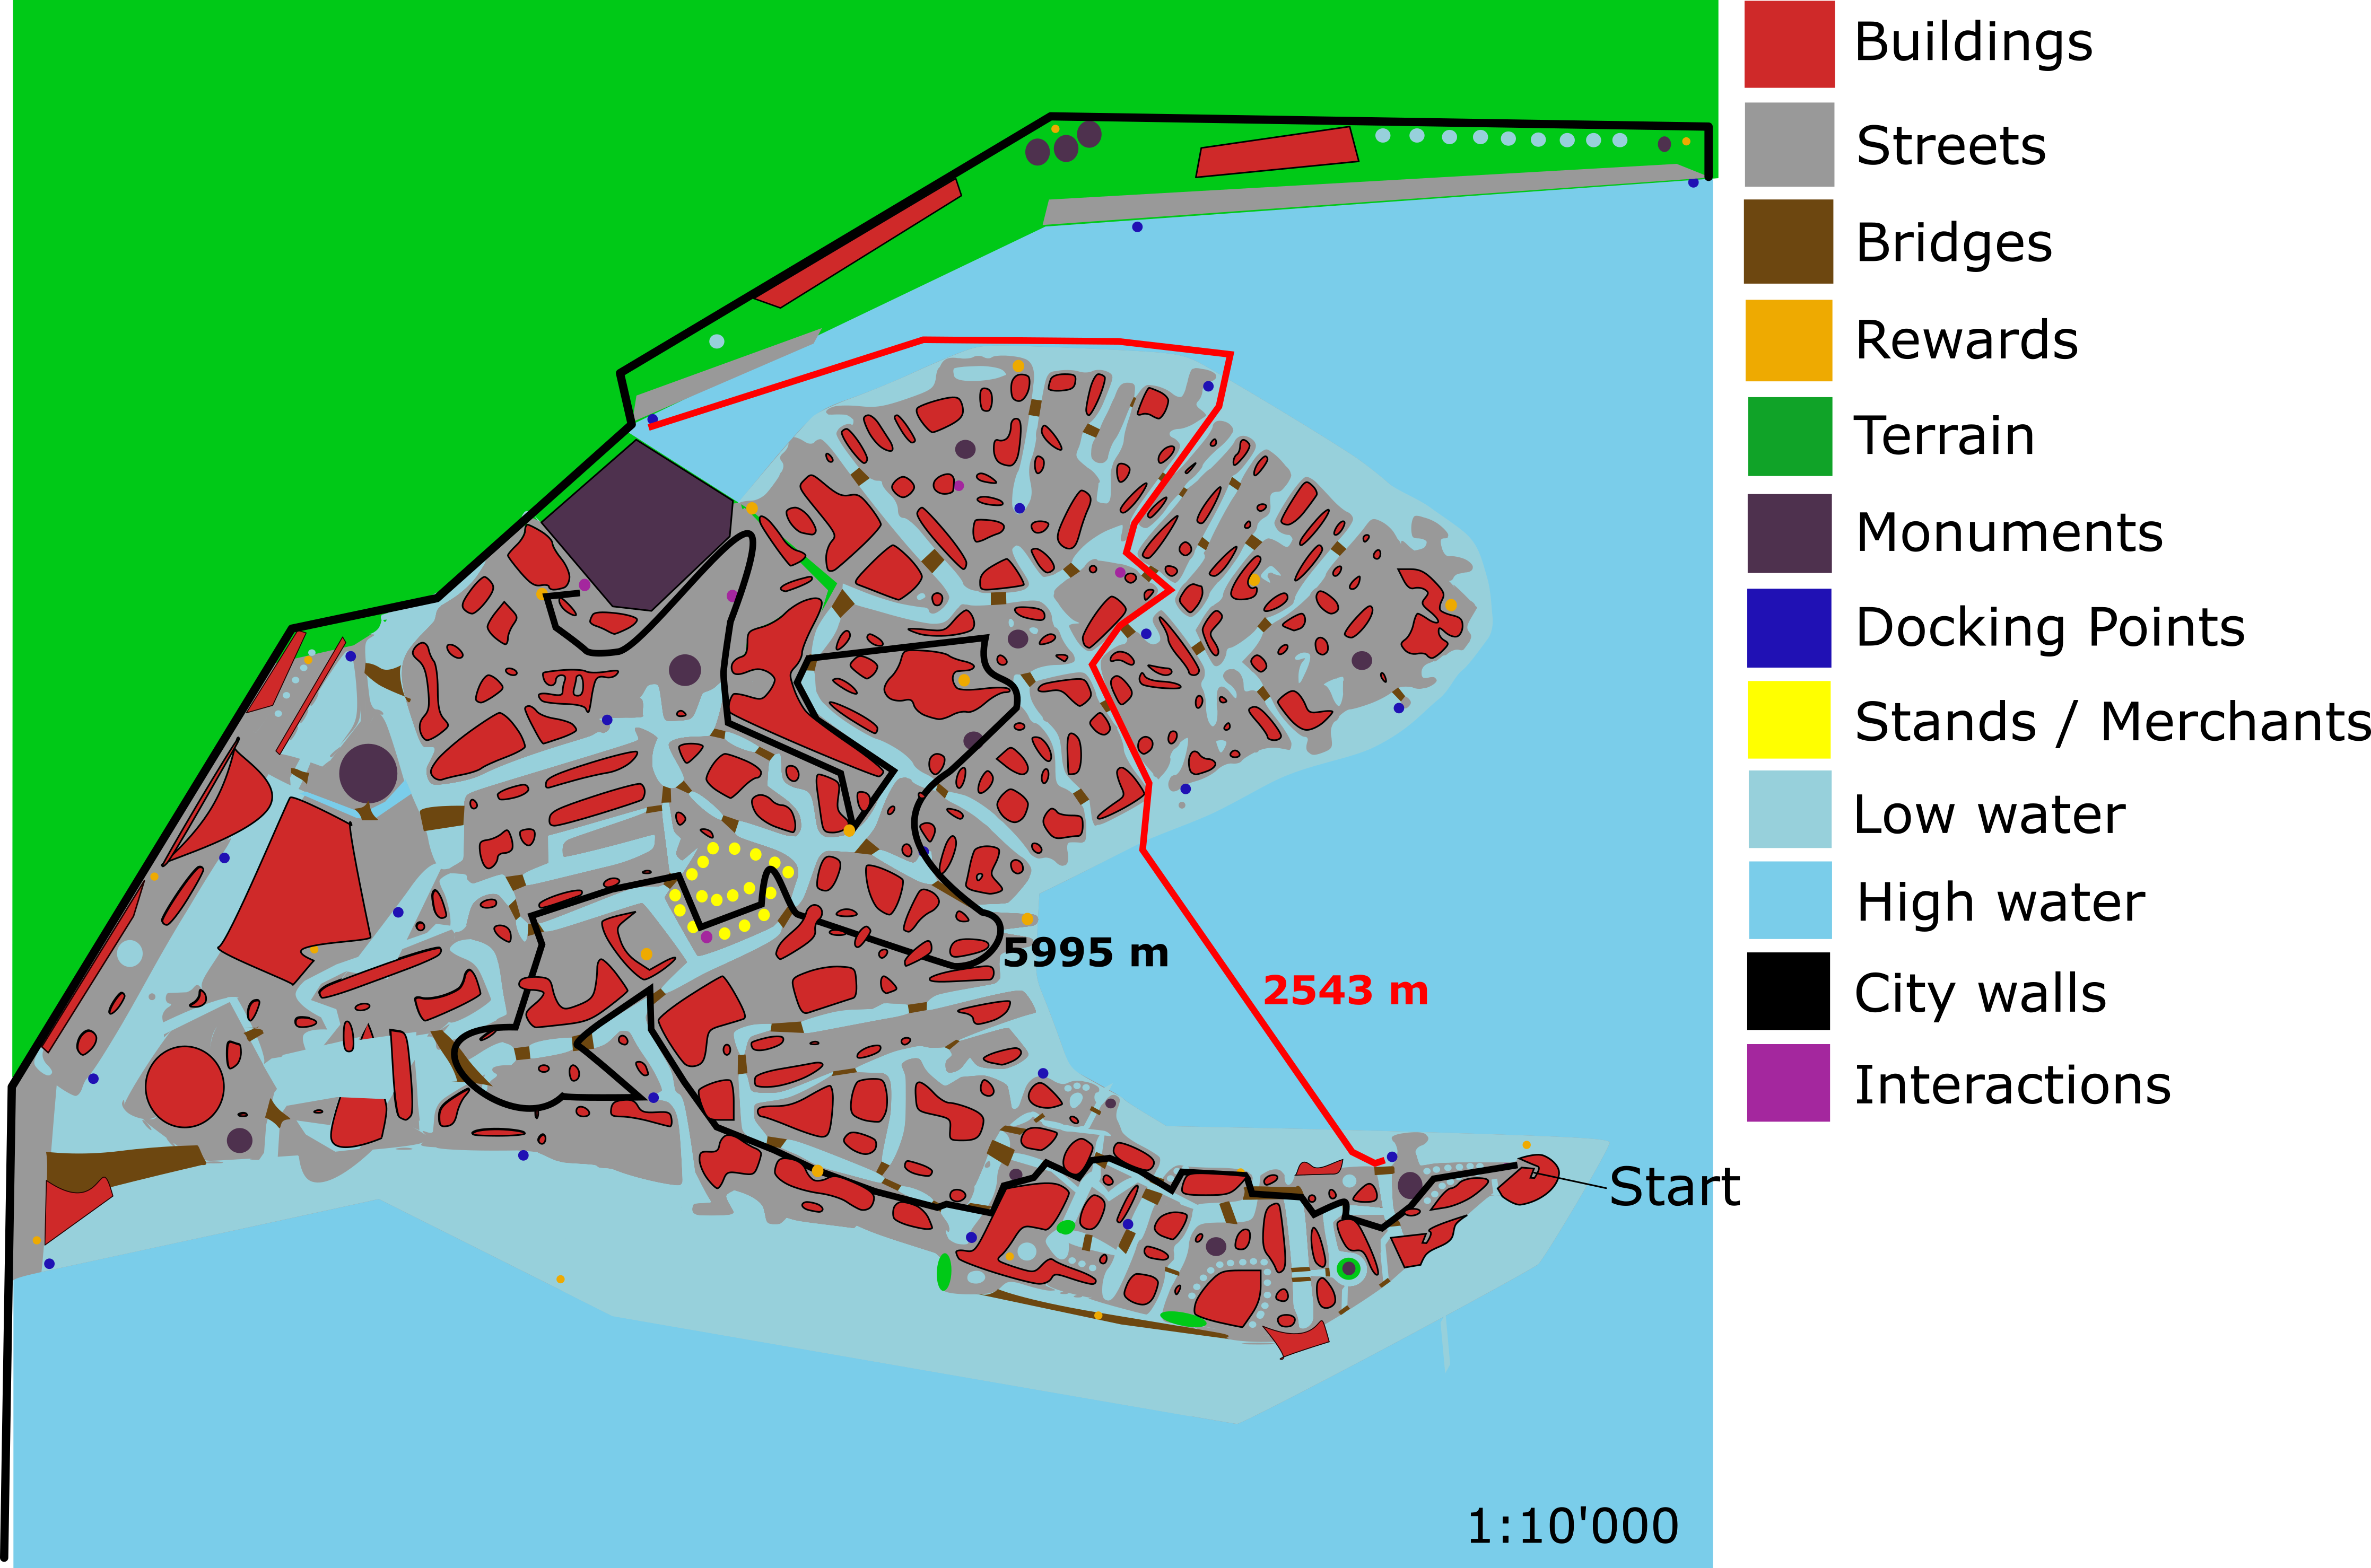
\includegraphics[width=\textwidth]{Images/Diagrams/dynamiapath2.png}
	\caption{Average path: $\sim$30 min}
\end{figure}

\begin{figure}[H]
    \centering
	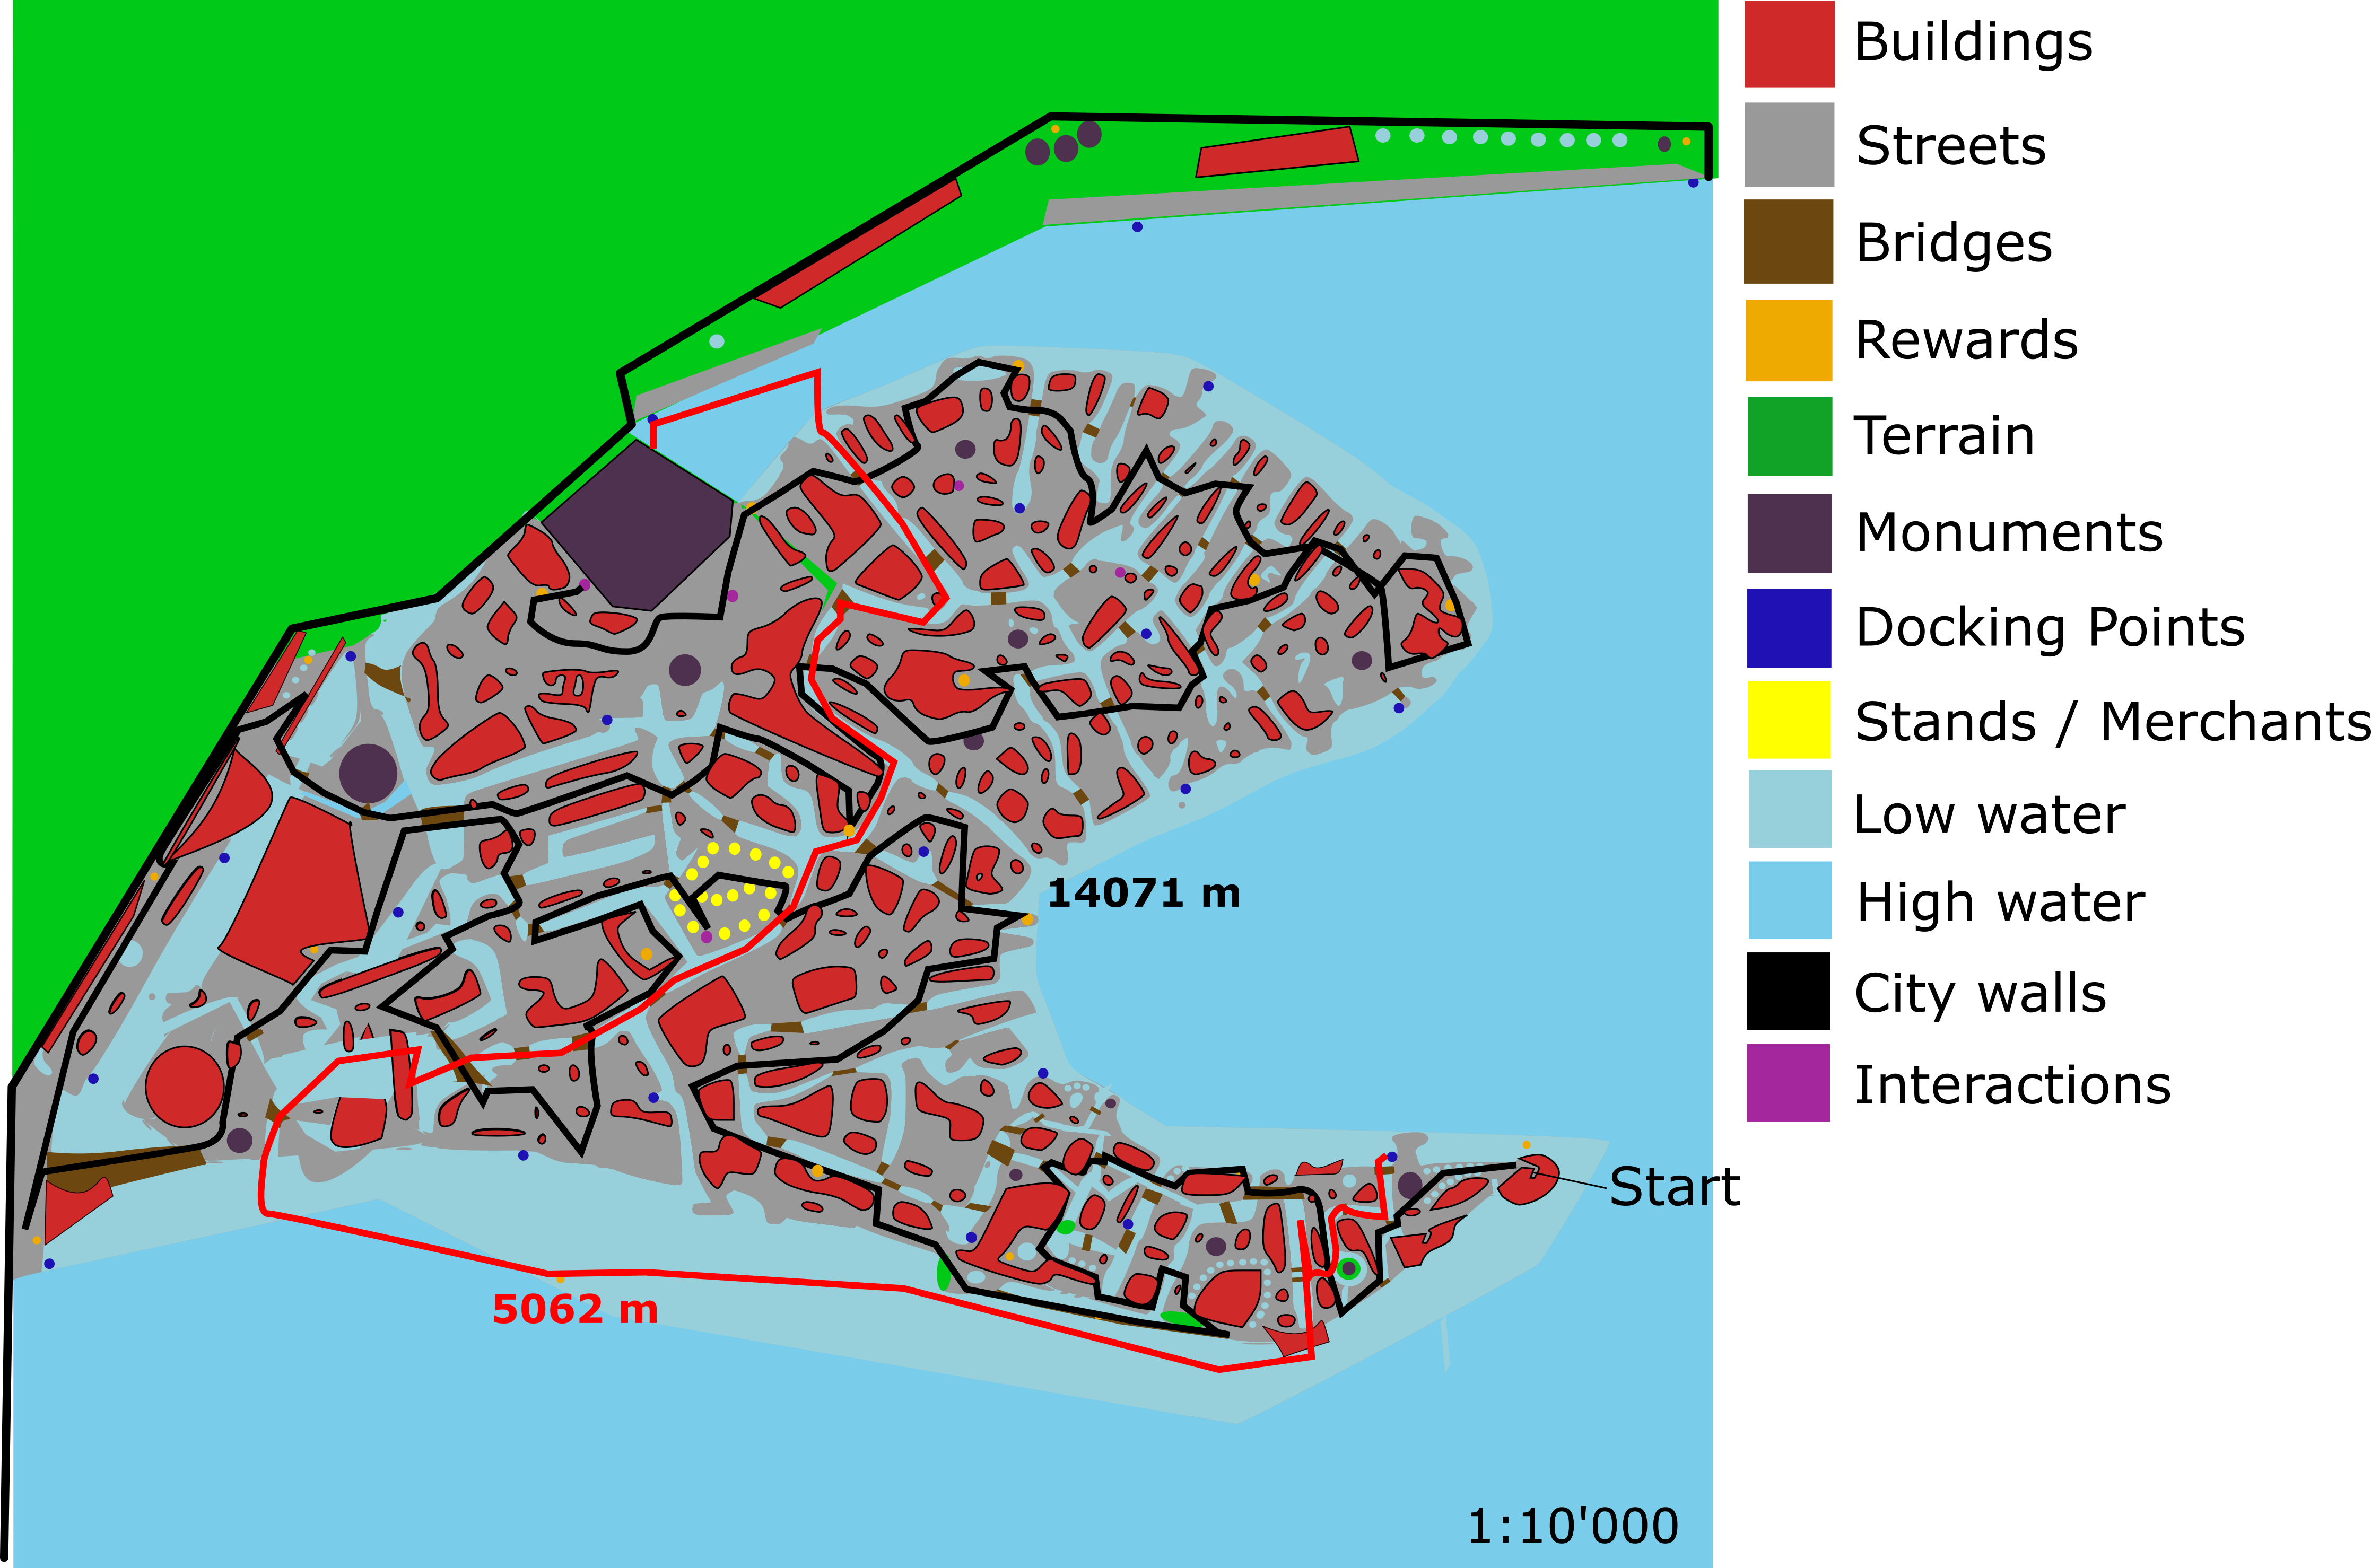
\includegraphics[width=\textwidth]{Images/Diagrams/dynamiapath3.png}
	\caption{Longest path: $\sim$71 min}
\end{figure}

The total expected time (assuming that the three different paths have equal probability) is about \textbf{90 minutes}.
